  \let\negmedspace\undefined
\let\negthickspace\undefined
\documentclass[journal]{IEEEtran}
\usepackage[a5paper, margin=10mm, onecolumn]{geometry}
\usepackage{lmodern} % Ensure lmodern is loaded for pdflatex
\usepackage{tfrupee} % Include tfrupee package

\setlength{\headheight}{1cm} % Set the height of the header box
\setlength{\headsep}{0mm}     % Set the distance between the header box and the top of the text

\usepackage{gvv-book}
\usepackage{gvv}
\usepackage{cite}
\usepackage{amsmath,amssymb,amsfonts,amsthm}
\usepackage{algorithmic}
\usepackage{graphicx}
\usepackage{textcomp}
\usepackage{xcolor}
\usepackage{txfonts}
\usepackage{listings}
\usepackage{enumitem}
\usepackage{mathtools}
\usepackage{gensymb}
\usepackage{comment}
\usepackage[breaklinks=true]{hyperref}
\usepackage{tkz-euclide} 
\usepackage{listings}                                      
\def\inputGnumericTable{}                                 
\usepackage[latin1]{inputenc}                                
\usepackage{color}                                            
\usepackage{array}                                            
\usepackage{longtable}
\usepackage{multicol}
\usepackage{calc}                                             
\usepackage{multirow}                                         
\usepackage{hhline}                                           
\usepackage{ifthen}                                           
\usepackage{lscape}
\begin{document}
	
	\bibliographystyle{IEEEtran}
	\vspace{3cm}
	
	\title{11.16.3.3.3}
	\author{EE24BTECH11030 - KEDARANANDA}
	% \maketitle
	% \newpage
	% \bigskip
	{\let\newpage\relax\maketitle}
	
	\renewcommand{\thefigure}{\theenumi}
	\renewcommand{\thetable}{\theenumi}
	\setlength{\intextsep}{10pt} % Space between text and floats
	
	
	\numberwithin{equation}{enumi}
	\numberwithin{figure}{enumi}
	\renewcommand{\thetable}{\theenumi}
	
	
	\textbf{Question}:\\
	A die is rolled, Find the probability that a number greater than or equal to one  will appear \\
	\textbf{Solution: }\\
	\textbf{Textual solution: }\\
	The probability of a given event 'A' (A: Outcome is greater than or equal to 1) can be calculated as follows: 
	\begin{align}
		\text{P(A)} = \frac{\text{Number of favorable outcomes}}{\text{Total possible outcomes}}
	\end{align}
	Since all outcomes on a standard die (\(1, 2, 3, 4, 5, 6\)) are greater than or equal to 1, all outcomes are favorable.
	
	\begin{align}
		\text{P(A)} = \frac{6}{6} = 1
	\end{align}
	
	\textbf{Computational solution: }\\
	\section*{Introduction}
	This document describes a computational experiment where a six-sided die is rolled 10,000 times. The outcomes are stored in a shared file, and Python is used to analyze these outcomes. The analysis calculates the probabilities of specific results (\( \geq 1, =1, =2, =3, =4, =5, =6 \)) and visualizes the probabilities using a stem plot.
	
	The workflow consists of two main parts:
	\begin{itemize}
		\item Generating random die rolls using a C program and storing the results in a file.
		\item Analyzing and plotting the probabilities using Python.
	\end{itemize}
	
	\section*{C Code Description}
	The C program is responsible for simulating 10,000 rolls of a six-sided die. It utilizes the \texttt{rand()} function to generate random numbers between 1 and 6. These outcomes are then written to a file named \texttt{outcomes.so}.
	
	Key features of the C program:
	\begin{itemize}
		\item The random number generator is seeded using the current time to ensure variability in results.
		\item A loop runs 10,000 iterations to generate the required number of outcomes.
		\item Each generated outcome is written line by line to the output file.
	\end{itemize}
	
	The file \texttt{outcomes.so} serves as a bridge between the C and Python programs, enabling the latter to perform statistical analysis on the data.
	
	\section*{Python Code Description}
	The Python program reads the outcomes stored in \texttt{outcomes.so}, calculates probabilities for specific outcomes, and visualizes the results using a stem plot.
	
	Key steps in the Python program:
	\begin{itemize}
		\item Read the data from \texttt{outcomes.so} and store it in a list.
		\item Calculate the probability of each outcome (\( \geq 1, =1, =2, =3, =4, =5, =6 \)) by counting occurrences and dividing by the total number of outcomes.
		\item Use the Matplotlib library to create a stem plot where:
		\begin{itemize}
			\item The x-axis represents the outcome categories (\( \geq 1, =1, =2, =3, =4, =5, =6 \)).
			\item The y-axis represents the probabilities, ranging from 0 to 1.
		\end{itemize}
	\end{itemize}
	
	The stem plot provides a clear visualization of the distribution of outcomes, making it easy to interpret the results.
	
	\section*{Graphical Output}
	The graphical output consists of a stem plot that shows the probability distribution of the die roll outcomes. The probabilities are calculated based on the 10,000 simulated rolls.
	
	Key observations from the plot:
	\begin{itemize}
		\item The probability of \( \geq 1 \) is always 1, as all outcomes are between 1 and 6.
		\item The probabilities for \( =1, =2, =3, =4, =5, =6 \) are approximately equal, reflecting the fairness of the die.
	\end{itemize}
	
	The stem plot serves as a visual summary of the experiment, highlighting the uniform probability distribution of a fair six-sided die.
	\begin{figure}[h!]
		\centering
		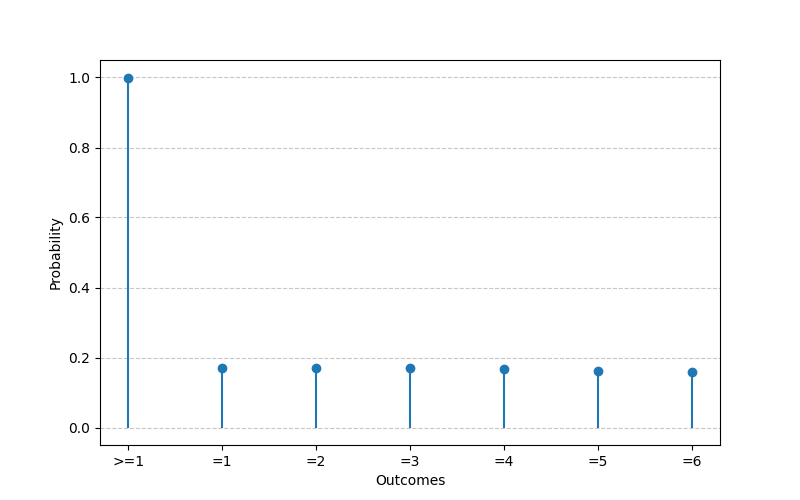
\includegraphics[width=\columnwidth]{figs/Fig.png}
		\caption{Solution of the system of linear equations}
		\label{stemplot}
	\end{figure}
	
\end{document}  